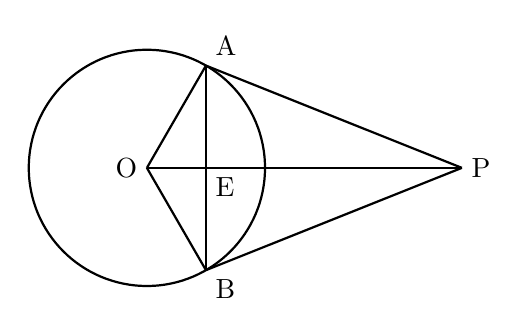
\begin{tikzpicture}[scale=1]

  % Define the center of the circle
  \coordinate (O) at (0,0);

  % Define the radius of the circle
  \def\R{1.5}

  % Draw the circle
  \draw[thick] (O) circle (\R);

  % Define points A and B on the circle
  \coordinate (A) at (60:\R);
  \coordinate (B) at (-60:\R);

  % Define point P outside the circle
  % The exact coordinates are approximate to match the image proportions
  \coordinate (P) at (4,0);
  
  % Define the intersection point E on OP and AB
  \coordinate (E) at (0.75,0);

  % Draw the tangents PA and PB
  \draw[thick] (P) -- (A);
  \draw[thick] (P) -- (B);

  % Draw the radius lines OA and OB
  \draw[thick] (O) -- (A);
  \draw[thick] (O) -- (B);

  % Draw the chord AB
  \draw[thick] (A) -- (B);
  
  % Draw the line segment OP
  \draw[thick] (O) -- (P);

  % Add labels for the points
  \node[left] at (O) {O};
  \node[above right] at (A) {A};
  \node[below right] at (B) {B};
  \node[right] at (P) {P};
  \node[below right] at (E) {E};

\end{tikzpicture}